\chapter{Discussion}\label{ch:discussion}

\begin{chapterabstract}
    This chapter begins with the outline of the work done as part of this thesis.
    This is followed up with the discussion of the individual results presented in Chapter~\ref{ch:results}.
    Follows up the discussion of other discovered aspects of the Gaia-X ecosystem.
    The chapter concludes with a section answering the thesis's research questions.
\end{chapterabstract}

\section{Outline}\label{sec:discussion_outline}

This thesis examined the ideas of federated ecosystems, data spaces and related concepts, special emphasis was placed on the concrete implementation of these ideas --- Gaia-X~\cite{gaiax}.
The goal of this work was to implement a Gaia-X-compliant data exchange module into the platform Carecentive~\cite{carecentive} based on available Gaia-X specifications and leveraging reference implementations and running services.

The implementation process of the data exchange module, acting as a proof of concept, itself served as a way to answer research question 2 --- ``\textit{What are the technical challenges in implementing Gaia-X-compliant software?}''.
The functionality of the implementation, Gaia-X services, and the specifications themselves are explored by running predefined experiments focused on different aspects of the data exchange process.
Those are used to answer research question 1 --- ``\textit{Is it feasible to share healthcare data in Gaia-X Data Spaces?}''.

\section{Proof of concept implementation}\label{sec:proof-of-concept-implementation}

As part of the practical side of the thesis was to implement a Gaia-X-compliant data exchange module into the Carecentive platform.
The reasoning behind this was twofold: (1) to enable the exchange of the palliative care trial data with other parties in a trustworthy and interoperable environment and (2) to assess the current state of the Gaia-X ecosystem and note any technical challenges in the process.

Therefore, a solution was developed and embedded into the Carecentive app to enable the registration of existing data assets into the Gaia-X ecosystem.
From a high level view, the module was supposed to serve two main functionalities.
Firstly, create the Gaia-X Credentials corresponding to objects in Carecentive; this includes mainly the Participant credential (corresponding to the Carecentive admin) and the credentials describing the offered data.
Secondly, the goal was to enable some kind of process (contracting, handshake, etc.), serving as a basis for the subsequent data exchange.

During the development, it quickly became clear that the implementation process was not going to be smooth.
The reasons for are related to the state of the specifications, reference implementation (XFSC) and the GXDCH services, the specific issues are discussed in the remaining parts of this section.

\subsection{Specifications}\label{subsec:specifications}

When people first familiarize themselves with Gaia-X's technical and functional specifics, they must decide which specification to review.
This is because the specifications are divided into five different documents; ``Policy Rules Conformity Document''~\cite{gaiax_policy_rules}, ``Architecture Document''~\cite{gaiax_architecture_document}, ``Trust Framework''~\cite{gaiax_trust_framework}, ``Identity and Access Management''~\cite{gaiax_identity_and_access_management}, and ``Data Exchange Document''~\cite{gaiax_data_exchange_document}.
The overview of available specifications is available in Figure~\ref{fig:specifications}.
Initially, it can be very confusing and unclear which document deals with the person's use-case, which leads to the need of studying multiple vast documents.

\begin{figure}
    \centering
    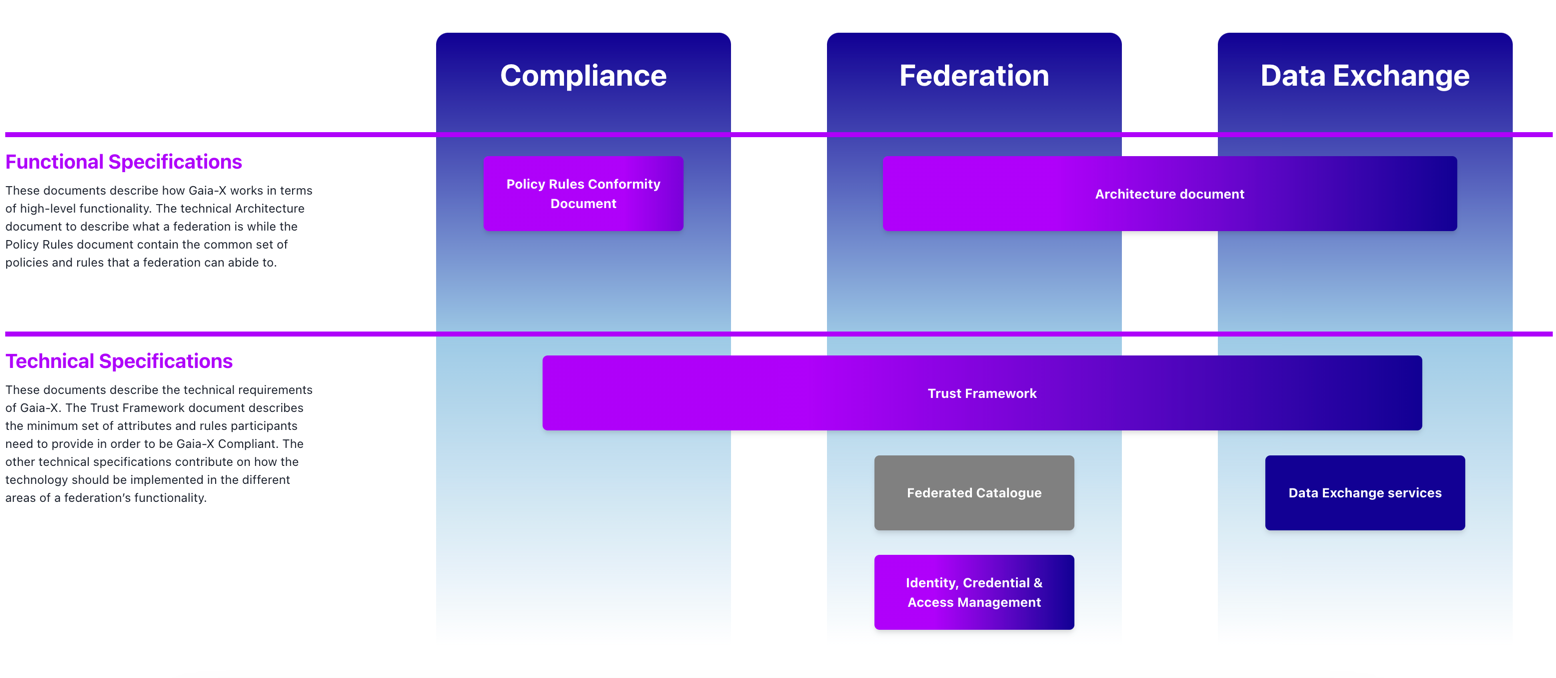
\includegraphics[width=\textwidth]{figures/specifications.png}
    \caption{Gaia-X specifications divided into functional and technical groups and ``Compliance'', ``Federation'' and ``Data Exchange'' blocs~\cite{gaiax}.}\label{fig:specifications}
\end{figure}

The issue that arises from this division and because the same components are often described in multiple different documents, this leads to inconsistencies.
For example, the \textit{DataProductDescription} credential described by the ``Data Exchange Document''~\cite{gaiax_data_exchange_document} is supposed to be inheriting attributes of the \textit{ServiceOffering} credential, defined in the ``Trust Framework''~\cite{gaiax_trust_framework}, but the common attributes do not match.
Following is an example of mismatched attributes in the format (\textit{service offering attributes}) vs. (\textit{data product description attributes}): (\texttt{name}, \texttt{policy}) vs. (\texttt{title}, \texttt{hasPolicy}) respectively.

Another issue with the ``Data Exchange Document''~\cite{gaiax_data_exchange_document} specification is a wording mismatch between the component in the specification (\textit{DataProduct}) and in the XFSC implementation of DCT (Data Contract Transaction) service (\textit{DataAsset}).
Yet another inconsistency surrounding the specifications relates to the policies.
The ``Data Exchange Document''~\cite{gaiax_data_exchange_document} states the allowed policy languages to be \textit{Rego}, \textit{ORDL}, and \textit{XACML}\footnote{\url{https://groups.oasis-open.org/communities/tc-community-home2?CommunityKey=67afe552-0921-49b7-9a85-018dc7d3ef1d}}, whereas other documents only mention \textit{Rego} and \textit{ORDL}.
Additionally, the \textit{Rego} policies are evaluated against a given input, but in the case of Gaia-X, it's unclear what attributes are part of the input object and I wasn't able to find the definition in any one of the specifications.

The specifications are also often vague about posed requirements.
Normally the objects' attributes are defined in tables and can be standalone Gaia-X credentials or just objects, which are part of the credentials, and this distinction is not always clear.
For example, normally when the ``Trust Framework''~\cite{gaiax_trust_framework} defines a link to another credential as the attribute using a comment like ``a resolvable link to the \texttt{credential} self-description providing the service''.
However the attribute \texttt{serviceAccessPoint} of \texttt{InstantiatedVirtualResource} is described as ``a list of Service Access Point which can be an endpoint as a mean to access and interact with the resource''.
This would imply a simple embedded object, but instead a link to the credential is expected.

I argue that Gaia-X should undertake efforts to remove the inconsistencies that exist between individual specifications.
Merging the different documents into a single large one could be beneficial to remove redundant definitions, which can cause inconsistencies.
Another approach could be creating an additional overarching document, which would explain the ``bigger picture'' of the Gaia-X ecosystem and explain the necessary components from the point of view of different user roles (Federator, Provider, Consumer).
A section on ``getting started'' with Gaia-X, which is commonly used by many software libraries and frameworks, along with minimal examples on the usage could bring a lot of value to newly onboarding users and smoothen-out the experience.

\subsection{Gaia-X Digital Clearing House}\label{subsec:gaia-x-digital-clearing-house}

The GXDCH is a set of running services consisting of Compliance, Notary, and Registry which are operationalizing the rules stated by the Gaia-X specifications.
As with the specifications, they are not free from their own set of issues.

The main issue is imperfect alignment with specifications.
For example, the Notary service, which currently only serves the purpose of validating LegalParticipant's registration number, issues a \textit{LegalRegistrationNumber} upon providing a valid registration number.
The ``Trust Framework''~\cite{gaiax_trust_framework} document specifies five admissible types of registration numbers --- \texttt{local} (state issued), \texttt{EUID}, \texttt{EORI}, \texttt{vatId}, and \texttt{leiCode}.
The Registry, which formalizes credential structure, recognizes \texttt{taxID} instead of the \texttt{local} registration number.
However, upon presenting state issued registration under either of these options, both lead to the Notary returning an error.

Other misalignment between the specifications and the formal Registry's implementation concerns the \texttt{LegalPerson} Gaia-X credential.
The attribute \texttt{legalAddress.countryCode} doesn't match the formalized version \texttt{legalAddress.countrySubdivisionCode}.

The formalized version of \texttt{DataResource} credential in the Registry's DB seems to be incorrectly aligned with the definition in the ``Trust Framework''~\cite{gaiax_trust_framework} specification.
In the document, the \texttt{exposedThrough} attribute expects a resolvable link to the \texttt{InstantiatedVirtualResource} credential, but the Registry expects a link to the \texttt{ServiceOffering} credentials.
This leads to the inability to obtain compliance for \texttt{DataResource}/\texttt{ServiceOffering}-related Gaia-X credentials.

Another major issue with the Registry and Compliance services is missing implementation of Gaia-X credentials defined in their respective specifications.
As and example ``Trust Framework''~\cite{gaiax_trust_framework} document defines two types of the Participant credential, \texttt{LegalPerson} and \texttt{NaturalPerson}, the Compliance and Registry services, however, only implement the \texttt{LegalPerson} at the moment.
The ``Architecture Document''~\cite{gaiax_architecture_document} also defines three roles for a Participant (Provider, Consumer, Federator), which are not yet implemented.
This is, however, acknowledged in the ``Trust Framework''~\cite{gaiax_trust_framework} specifications.

Importantly, the data exchange-related credentials are also not implemented in the Registry's trusted DB, which means that none of the credentials defined in the ``Data Exchange Document''~\cite{gaiax_data_exchange_document} cannot be validated and receive compliance.
Additionally, the possibility of notarizing the \texttt{DataProductUsageContract} credentials is another use-case described by the ``Data Exchange Document''~\cite{gaiax_data_exchange_document}, which is not implemented by the Notary.

One of the less severe, but still notable inconsistency is the naming of the GXDCH services' endpoints.
The compliance uses \texttt{kebab-case} for endpoint routes, the Notary uses \texttt{camelCase}, and the Registry combines both of the conventions.

I believe Gaia-X should work intensely on ensuring the implementation, including the formalization of the Credential vocabulary, conforms to the predefined specifications.
Clearly marking the features, which are not yet implemented and exist only as specifications, would help adopters immensely to save time and resources.

I also find the benefit of validating legal entity registration numbers debatable.
This is because the test only asserts the validity of said registration numbers and not their affiliation to the respective legal person.
This does little to help establish the trust among Participants and introduces a dependence on a centralized service (EU ran API is used for validating VAT ID).
During my implementation phase, the API for validation was oftentimes down, leading to the Compliance's service inability to provide compliance.

A feasible alternative may be validating a registration number based on the attributes included in the legal person's certificate.
This fits well to the Gaia-X's requirement to use qualified certificates regulated by the eIDAS Regulation (EU) No 910/2014, which stipulates that \textit{``Qualified certificates for electronic seals shall contain at least the name of the creator of the seal and, where applicable, registration number as stated in the official records;''}~\cite{eidas}.

\section{Cross Federation Services Components}\label{sec:cross-federation-services-components}

Cross Federation Services Components (XFSC) is the reference implementation of concepts and workflows as defined by Gaia-X specifications.
It includes the services operated by GXDCH,
It includes core services for data exchange (``Data Connector'') and for setting up federations, like the ``Core Catalogue Functions'', ``Orchestration''.
Additionally, they provide tools like the ``Self-Description Wizard'', ``Personal Credential Manager'', ``Organization Credential Manager'', and ``Data Exchange Logging Services''.
Different services are in a different state of the development phase as indicated visually on the Gaia-X website\cite{gaiax}.
Some services are still in development, as indicated by their box being greyed-out, others, like Compliance, Registry and Notarization services are already released.
The development status also differs by the selected version, where most of the services are developed in the version \texttt{21.03}.

The initial goal was to use the ``Data Connector'' service for data exchange between Carecentive and data consumer.
However, because the ``Data Connector'' service is not released in any of the versions, the focus was changed on providing data using Carecentive's existing API.
To enable data consumption over the existing API, the aim was to utilize the ``Data Contract Services'' for the initial handshake between Carecentive and the data consumer.

``Data Contract Services'' implement data exchange and contracting workflows as defined in the ``Data Exchange Document''~\cite{gaiax_data_exchange_document}.
The intent was to use the version \texttt{21.03}, since it's the only stated release of the service and integrate it into the running stack of Carecentive.
However, upon examining the service's repository and setting it up, it was discovered that while the service seems functional on the first look, the API has hardcoded responses to predefined requests.
In conclusion, crucial internal components are missing from the service, which renders the ``Data Contract Services'' unusable.

It is necessary to mention that coming up to this conclusion was hindered by the incorrectly visualized release status.
Furthermore, the visual representation of services links to an old Gitlab group, which was migrated to the Eclipse Foundation Gitlab account, leading to the need to search for the correct repository.
The links should be updated to redirect to the correct respective repositories and ideally to the correct branch or commit marking the release.
This would significantly simplify the adoption process for developers.
Additionally, the documentation/README files should be improved, as in the case of ``Data Contract Services'', the README file consists mostly of an unmodified template.

To mitigate this issue, a simplified version inspired by contracting workflow of the ``Data Exchange Document''~\cite{gaiax_data_exchange_document} was implemented directly into the Carecentive platform to enable data exchange functionality.
The exact workflow is detailed in Section~\ref{subsec:data-contracting}.
This unfortunately meant that I was unable to test features related to a missing policy engine like policy enforcement and contract negotiation.

Gaia-X should focus on providing correct information on the development status of XFSC services and update the links to lead to correct repositories.
Adopting developers would also benefit greatly from improved documentation of the XFSC services.

\section{Experiments}\label{sec:experiments_discussion}

Six experiments were designed to test the implementation of the data exchange module and to evaluate the feasibility of the Gaia-X ecosystem for exchanging data, particularly in the field of medical trials.
Out of the six tests, 3 were carried out successfully, 2 failed and 1 couldn't be conducted due to the missing XFSC component --- the ``Data Contract Services''.

The two failed experiments both were verifying the process of obtaining Gaia-X compliance for the data resource and data exchange-related Gaia-X Credentials.
Their failure showcases that the maturity of the Gaia-X project is low, as the concept of Gaia-X Credentials is a central part of the project.
The missing XFSC component leading to the inability to conduct experiment no.~6 also shows, the project is still very much in active development.

The experiment no.~1 demonstrates the very-core feature of onboarding Participants is functional, but currently is only limited to legal entities and not natural persons or other types of Participants.
It is unlikely that in the current developmental lifecycle the Gaia-X can accommodate non-trivial use-cases.

The test cases no.~4 and 5 showcase that data exchange is possible, but at the moment only with additional efforts in developing parts of the missing functionality or utilizing non-Gaia-X protocols.
These tests are evaluated as passed as they are based on Gaia-X specifications and lead to a successful exchange of data.
However, since they are based on credentials which could not be issued compliance for and therefore were not validated, the process cannot be though of as Gaia-X-compliant.
This is underlined by the fact that the key features advertised by the ``Data Contract Services'', such as policy enforcement and contract negotiation are not implemented in the simplified version of the contracting service.

To answer research question 1 --- ``\textit{Is it feasible to share healthcare data in Gaia-X Data Spaces?}'' --- the answer is currently no.
The reasons are the missing XSFC components and inconsistencies between specifications and running GXDCH services.

%TODO: metrics and risks?